
\documentclass{acm_proc_article-sp}

\begin{document}

\title{How Far have Cars driven the Nature!}

\numberofauthors{2} 
\author{
% 1st. author
\alignauthor
Amruta Chavan\\
       \affaddr{MS in Data Science at}\\
       \affaddr{Indiana University of Bloomington}\\
       \affaddr{GitLab ID: amchavan}
       \email{amchavan@iu.edu}
% 2nd. author
\alignauthor
Aditya Tanikanti\\
       \affaddr{MS in Data Science at}\\
       \affaddr{Indiana University of Bloomington}\\
       \affaddr{GitLab ID: aditya.tanikanti}
       \email{atanikan@iu.edu}
}
\toappear{}
\maketitle
\begin{abstract}
This paper provides an insight into the fuel consumption and carbon emission by different car models driven all over the world. It analyses and compares performance of different types of cars based on types,brands and other specifications.

This project will throw light on how much and how badly are automobiles affecting the environment and causing Global Warming. We will try to find some fuel efficient cars and/or alternate solutions to avoid further damage to nature. 
\end{abstract}

\section{Introduction}
Global warming endangers our health, jeopardizes our national security, and threatens other basic human needs. Some impacts-such as record high temperatures, rising seas, and severe flooding and droughts-are already increasingly common.

Our personal vehicles are a major cause of global warming. Collectively, cars and trucks account for nearly one-fifth of all US emissions, emitting around 24 pounds of carbon dioxide and other global-warming gases for every gallon of gas. About five pounds comes from the extraction, production, and delivery of the fuel, while the great bulk of heat-trapping emissions-more than 19 pounds per gallon-comes right out of a car's tailpipe.

In total, the US transportation sector-which includes cars, trucks, planes, trains, ships, and freight-produces nearly thirty percent of all US global warming emissions, more than almost any other sector.

While in EU, cars are responsible for around 12 percent of total emissions of carbon dioxide (CO2), the main greenhouse gas.

Unfortunately, oil-related emissions may rise in the coming years as the oil industry extracts and refines "unconventional" oils, such as tar sands and tight oil. Using less oil, avoiding unnecessary emission from the oil, finding alternative for fuel, cars etc are few steps towards preventing global warming that this project will try focus on. \cite{ConcernedScientists2014}

\section{Data Sets}
This project uses dataset published by US-EPA \textit{United States Environment Protection Agency}. Also we will be combining dataset from various resources to obtain more detailed analysis.Dataset links, can be found in the references as
\cite{2014}, \cite{2015}


\section{Technologies}
We intend to use the following technologies in our project

a) Python/Ipython Notebook(Anaconda) - For Data Cleaning/Wrangling, Exploratory Data Analysis and modeling data so as to predict CO2 emission rates. \\
b) PySpark to implement the modeling part in a map reduce format and to store the data in HDFS\\
c) D3.js - Visualizing the graphs we generated via the exploratory data analysis phase\\
d) futuresystems/chameleoncloud - To further speed up the modelling phase if required.

\section{Proposal}
All new cars and light trucks sold in the U.S. are required to have a economy label posted on the window sticker. The label contains the city and highway miles-per-gallon values, as well as other related information. To calculate these values, laboratory tests are performed on pre-production vehicles.
We will be reviewing and analysing the data from this testing and predicting most efficient vehicles to purchase that could reduce fuel emission.

We will be studying performance of various car models that have been launched since 1984-2017 and how their usage has been affecting environment.

The project will compare cars based on brands(Fiat, Honda, Mini, Rolls Royce etc), models(sedan, SUV, mid-sized, full-sized, compact etc) and other factors within these models that are affecting the environment adversely. We will also try and build a model and use machine learning algorithms so as to predict the emission value(CO2) given cars details.

\section{Artifacts}

We performed preliminary analysis on the data set to plot graphs in Python to understand the fuel efficiency and carbon emission by selected car models as shown in the graphs below.


\begin{figure}
\centering
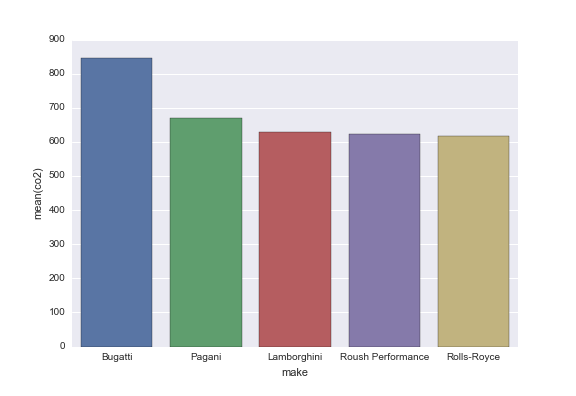
\includegraphics[height=4in, width=3.5in]{highco2}
\caption{Highest level of CO2 Emissions by different Car Brands}
\end{figure}

\begin{figure}
\centering
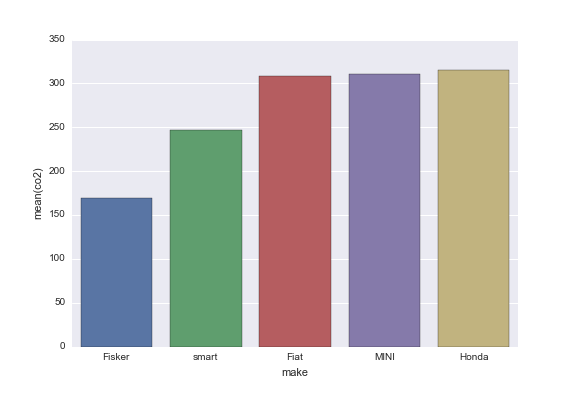
\includegraphics[height=4in, width=3.5in]{lowco2}
\caption{Lowest level of CO2 Emissions by different Car Brands}
\end{figure}

\begin{figure}
\centering
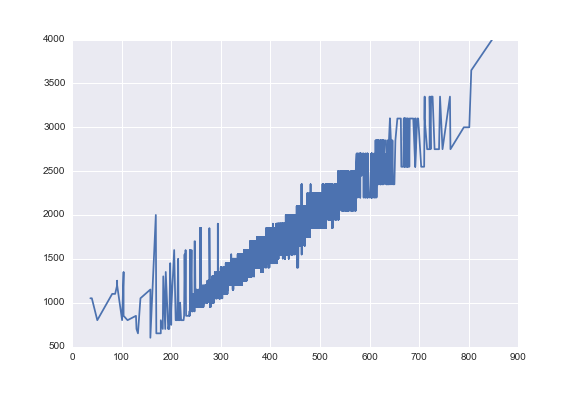
\includegraphics[height=4in, width=3.5in]{co2vsfuel}
\caption{CO2 emission vs Fuel Cost}
\end{figure}

Our project will include similar analysis and comparisons between various car specifications and fuel consumption to find efficient and economic solutions to reduce causes of global warming.

\section{Conclusion and Future Scope}
We will try to compare cars across different models, brands and prices to find correlation between fuel consumption and cost efficient models.
Through this project we will try to come to conclusion and possibly find efficient way to reduce car usage thereby contributing towards environment friendly solutions to commute.

\bibliographystyle{abbrv}
\bibliography{sample}

\end{document}
